\documentclass{beamer}
\usepackage{bbm}
\usepackage{algorithm}
\usepackage{algpseudocode}
\usepackage{tikz}
\usepackage{amsmath}
\usepackage{amssymb}
\usepackage{array}
\usepackage{graphicx}
\graphicspath{{figures/}} % Added to ensure the figures directory is searched
\usepackage{capt-of} % Added to enable captionof in beamer

% Theme choice:
\usetheme{Madrid}

% Title page details:
\title{A Petri Nets Model for Blockchain Analysis}
\subtitle{Seminar for the course of CMCS}
\author{Luca Lombardo}
\date{}

\begin{document}

\begin{frame}[plain]
    \titlepage
    \begin{center}
        \footnotesize{\textit{Based on the work of: Andrea Pinna, Roberto Tonelli, Matteo Orr\'{u}, Michele Marchesi}}
    \end{center}
\end{frame}

% Outline frame
\begin{frame}{Structure of the Presentation}
    \tableofcontents
\end{frame}

\section{Introduction: A Petri Net Model for Blockchain Analysis}
\label{sec:Intro}
\begin{frame}{A Petri Net Model for Blockchain Analysis}
    \footnotesize

    \begin{block}{Key Contributions}
        \begin{itemize}
            \item \textbf{Addresses Petri Net (APN):} Maps Bitcoin addresses to \textit{places} and transactions to \textit{transitions} in a P/T Net
            \item \textbf{Entities Petri Net (EPN):} Groups addresses into owner entities using a clustering algorithm
        \end{itemize}
    \end{block}

    \vspace{-0.2cm}
    \begin{block}{Advantages of PN Formalism}
        \begin{itemize}
            \item Algebraic structure enables formal analysis of transaction patterns
            \item Native representation of blockchain architecture through PN semantics
            \item Enables dynamic simulations for network behavior forecasting
        \end{itemize}
    \end{block}

    \vspace{-0.2cm}
    \begin{columns}[T]
        \begin{column}{0.5\textwidth}
            \textbf{Model Features}
            \begin{itemize}
                \item Preserves transaction topology
                \item Supports address clustering
                \item Enables multi-scale analysis
            \end{itemize}
        \end{column}

        \begin{column}{0.5\textwidth}
            \textbf{Paper Structure}
            \begin{itemize}
                \item System overview
                \item PN model definition
                \item APN/EPN construction
                \item Blockchain analysis results
            \end{itemize}
        \end{column}
    \end{columns}
\end{frame}

\begin{frame}{Bitcoin Blockchain: Architecture \& Transactions}
    \footnotesize
    \vspace{-0.2cm}
    \begin{block}{Overview}
        \begin{itemize}
            \item \textbf{Distributed Public Ledger:} A global database that stores every validated Bitcoin transaction.
            \item \textbf{Chain of Blocks:} Transactions are grouped into blocks that form an ordered sequence (the Blockchain).
        \end{itemize}
    \end{block}

    \vspace{-0.2cm}
    \begin{block}{Transaction Structure}
        \begin{itemize}
            \item \textbf{Inputs:} Reference previous unspent outputs (UTXOs) from earlier transactions.
            \item \textbf{Outputs:} List one or more addresses (e.g., strings starting with "1" or "4") along with their associated values.
            \item \textbf{UTXO Model:} An address's balance equals the sum of its unspent outputs.
        \end{itemize}
    \end{block}

    \vspace{-0.2cm}
    \begin{block}{User Interaction}
        \begin{itemize}
            \item \textbf{Digital Wallets:} Bitcoin clients store public/private key pairs that manage one or more addresses.
            \item \textbf{Anonymity:} Only addresses are recorded; no personal identity information is required.
        \end{itemize}
    \end{block}
\end{frame}

\subsection{Bitcoin Blockchain}
\begin{frame}{Bitcoin Blockchain: Architecture \& Transactions}
    \centering
    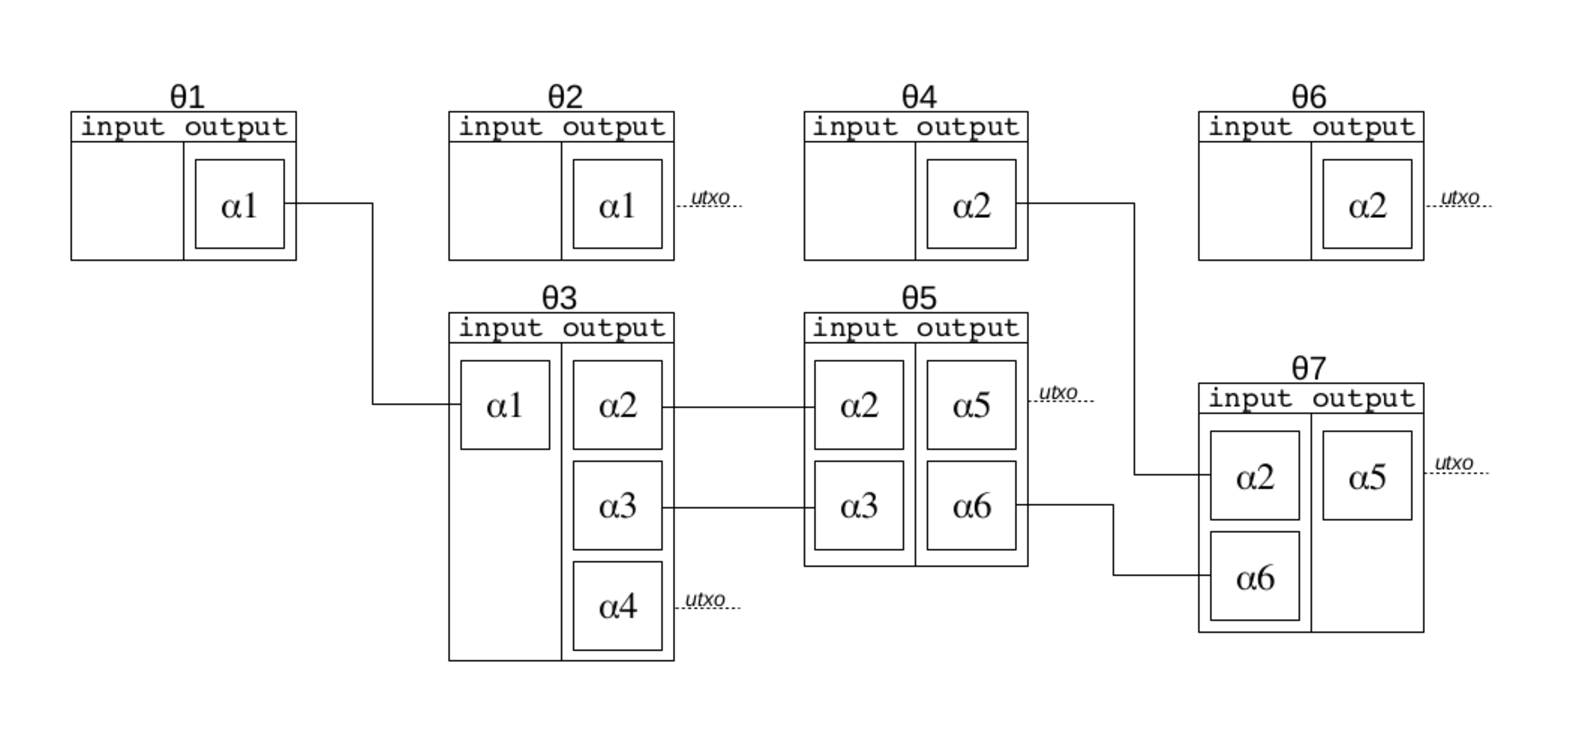
\includegraphics[width=1\linewidth]{ReteEsempio_1}
    \captionof{figure}{Simplified transaction schema}
\end{frame}

\begin{frame}{Bitcoin Blockchain: Transaction Verification \& Mining}
    \footnotesize

    \begin{block}{Transaction Validation}
        \begin{itemize}
            \item \textbf{Broadcast \& Pending:} Transactions are shared in the peer-to-peer network and wait to be validated.
            \item \textbf{Validation Rules:}
                  \begin{itemize}
                      \item Each input must reference a valid UTXO.
                      \item The total value of outputs must not exceed that of inputs.
                  \end{itemize}
        \end{itemize}
    \end{block}

    \begin{block}{Mining Process}
        \begin{itemize}
            \item \textbf{Proof-of-Work:} Miners solve a computational puzzle by finding a hash.
            \item \textbf{Block Contents:} A block includes the selected transactions, the previous block's hash, its block height, and miner information.
            \item \textbf{Incentives:} The first miner to solve the puzzle receives a block reward
        \end{itemize}
    \end{block}

    % \begin{block}{Network Dynamics}
    %     \begin{itemize}
    %         \item \textbf{Consensus Mechanism:} Full nodes verify blocks and the network adopts the longest chain.
    %         \item \textbf{Difficulty Adjustment:} The mining challenge is periodically adjusted to maintain an average of one new block every ten minutes.
    %         \item \textbf{Mining Pools:} Miners often collaborate in pools to optimize their chances of winning the reward.
    %     \end{itemize}
    % \end{block}
\end{frame}

\subsection{Petri Nets: an overview}
\begin{frame}{Petri Nets: Basic Concepts}
    \footnotesize
    \begin{block}{Overview}
        A \textbf{Petri Net} is a formal model for distributed systems built on a bipartite graph consisting of:
        \begin{itemize}
            \item \textbf{Places:} Represent conditions, resources, or system states.
            \item \textbf{Transitions:} Represent events that change these states.
        \end{itemize}
    \end{block}

    \begin{block}{Graph Structure}
        \begin{itemize}
            \item \textbf{Bipartite Graph:} Only two types of nodes are allowed, and connections occur only between nodes of different types.
            \item \textbf{Arcs:} Directed arcs link places and transitions:
                  \begin{itemize}
                      \item \textit{Pre-arcs:} Arcs from places to transitions (inputs).
                      \item \textit{Post-arcs:} Arcs from transitions to places (outputs).
                  \end{itemize}
        \end{itemize}
    \end{block}
\end{frame}

\begin{frame}{Petri Nets: Algebraic Formalism \& Markings}
    \footnotesize
    \begin{block}{Algebraic Description}
        A Petri Net is formally defined as a quadruple:
        \[
            N = (P, T, Pre, Post)
        \]
        where:
        \begin{itemize}
            \item \(P=\{p_1, p_2, \dots, p_m\}\) is the set of places.
            \item \(T=\{t_1, t_2, \dots, t_n\}\) is the set of transitions.
            \item \(Pre: P \times T \rightarrow \mathbb{N}\) is the \emph{pre-incidence} function.
            \item \(Post: P \times T \rightarrow \mathbb{N}\) is the \emph{post-incidence} function.
        \end{itemize}
        These incidence functions are typically represented as \(m \times n\) matrices.
    \end{block}

\end{frame}

\begin{frame}
    \frametitle{Petri Nets: Algebraic Formalism \& Markings}

    \begin{block}{Markings \& Firing Rule}
        \begin{itemize}
            \item A \textbf{marking} \(M\) is a vector assigning tokens to places, thus representing the system state.
            \item \textbf{Firing:} When a transition fires, it:
                  \begin{enumerate}
                      \item Consumes tokens from its pre-connected places.
                      \item Produces tokens in its post-connected places.
                  \end{enumerate}
            \item The complete system is denoted as \(\langle N, \mathbf{M}_0 \rangle\), where \(\mathbf{M}_0\) is the initial marking.
            \item In our work on Blockchain analysis, we focus on the net structure, without defining a specific marking.
        \end{itemize}
    \end{block}

\end{frame}

\section{Address Petri Net}
\begin{frame}{Addresses Petri Net: Overview and Definitions}
    \footnotesize
    \begin{block}{Motivation}
        \begin{itemize}
            \item Blockchain transactions move bitcoins between addresses.
            \item The inherent bipartite structure (addresses and transactions) suggests a natural mapping to a Petri Net.
        \end{itemize}
    \end{block}

    \begin{block}{Definitions}
        \begin{itemize}
            \item \(\mathcal{A}=\{\alpha_1,\alpha_2,\dots,\alpha_m\}\): Finite set of addresses (inputs/outputs).
            \item \(\Theta=\{\theta_1,\theta_2,\dots,\theta_n\}\): Set of validated transactions.
        \end{itemize}
    \end{block}

    \begin{block}{Addresses Petri Net Structure}
        \begin{itemize}
            \item Define \(N_\alpha = (P_{\alpha}, T, \mathbf{PreA}, \mathbf{PostA})\) where:
                  \begin{itemize}
                      \item \(P_{\alpha} = \{p\alpha_1, p\alpha_2, \dots, p\alpha_m\}\) associates one place per address.
                      \item \(T = \{t_1, t_2, \dots, t_n\}\) associates one transition per transaction.
                      \item \(\mathbf{PreA}\) and \(\mathbf{PostA}\) are the pre- and post-incidence matrices.
                  \end{itemize}
            \item These sets are built by scanning the Blockchain for new addresses and transactions.
        \end{itemize}
    \end{block}
\end{frame}

\begin{frame}{Addresses Petri Net: Constructing the Incidence Matrices}
    \footnotesize
    \begin{block}{Transaction Representation}
        \begin{itemize}
            \item Each transaction \(\theta\) is split into:
                  \begin{itemize}
                      \item \(\textbf{In}(\theta) \subseteq \mathcal{A}\): Set of input addresses.
                      \item \(\textbf{Out}(\theta) \subseteq \mathcal{A}\): Set of output addresses.
                  \end{itemize}
            \item The corresponding transition \(t\) represents \(\theta\) in the Petri Net.
        \end{itemize}
    \end{block}

    \begin{block}{Matrix Construction}
        \begin{itemize}
            \item For every \(\alpha \in \textbf{In}(\theta)\):
                  \begin{itemize}
                      \item Add a \textbf{pre-arc} from place \(p\alpha\) to transition \(t\).
                      \item Set \(\mathbf{PreA}(p\alpha, t)=1\).
                  \end{itemize}
            \item For every \(\alpha \in \textbf{Out}(\theta)\):
                  \begin{itemize}
                      \item Add a \textbf{post-arc} from transition \(t\) to place \(p\alpha\).
                      \item Set \(\mathbf{PostA}(p\alpha, t)=1\).
                  \end{itemize}
            \item The matrices \(\mathbf{PreA}\) and \(\mathbf{PostA}\) are of dimension \(m\times n\).
        \end{itemize}
    \end{block}
\end{frame}

\begin{frame}{Addresses Petri Net: Example and Analysis}
    \footnotesize
    \vspace{-0.2cm}
    \begin{block}{Example Overview}
        \begin{itemize}
            \item Consider a simplified set of transactions (e.g. as in the previous slide)
            \item The Addresses Petri Net has:
                  \begin{itemize}
                      \item 6 places (\(P_{\alpha} = \{p\alpha_1, \dots, p\alpha_6\}\)).
                      \item 7 transitions (\(T = \{t_1, \dots, t_7\}\)).
                  \end{itemize}
        \end{itemize}
        Below a graphical representation of an addresses Petri Net equivalent to the
        simplified transaction chains.
    \end{block}
    \begin{center}
        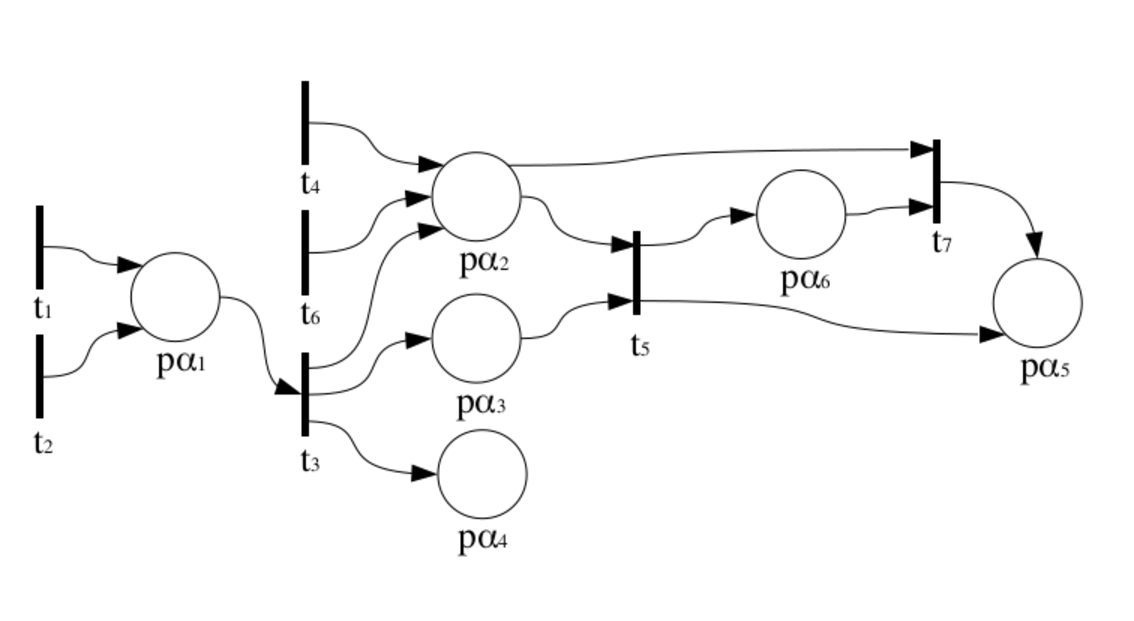
\includegraphics[width=0.7\linewidth]{ReteEsempio_1pt}\label{fig:ReteEsempio_1pt}

    \end{center}

\end{frame}

\begin{frame}
    \frametitle{Address Petri Nets:
    \begin{block}{Incidence Matrices and Analysis}
        \begin{itemize}
            \item \textbf{Pre-incidence matrix \(\mathbf{PreA}\):} Captures the number of times an address appears as an input.
            \item \textbf{Post-incidence matrix \(\mathbf{PostA}\):} Captures the outputs associated with each transaction.
            \item By computing the difference (\(\mathbf{PostA} - \mathbf{PreA}\)) for each row, one can:
                  \begin{itemize}
                      \item Determine the number of UTXOs per address.
                      \item Infer whether an address balance is null (zero tokens).
                  \end{itemize}
            \item Transactions sharing identical input and output sets may be merged into one transition with a firing clock, aiding dynamic analyses.
        \end{itemize}
    \end{block}

\end{frame}

\end{document}
